\documentclass[../../algebra.tex]{subfiles}
\usepackage{tikz}
\usepackage{amsmath}
\usetikzlibrary{calc}

\usetkzlibrary{angles}
\setcounter{secnumdepth}{3} % 让三级标题有编号
\setcounter{tocdepth}{3}    % 目录显示到三级标题
\renewcommand{\thesubsubsection}{\arabic{subsubsection}} 
\begin{document}
\subsubsection{最值问题}

如图,在 $\triangle ABC$ 中,$CA = CB = 5$,$AB = 6$,$D$ 为 $AB$ 边上一动点,连接 $CD$,将 $CD$ 绕点 $C$ 逆时针旋转到 $CE$,使 $\angle ACB = \angle DCE$。连接 $DE$ 交 $BC$ 于点 $F$。则 $CF$ 的最小值为\underline{\quad\quad\quad}。

\vspace{1em}
\begin{center}
    \begin{minipage}{0.45\textwidth}
        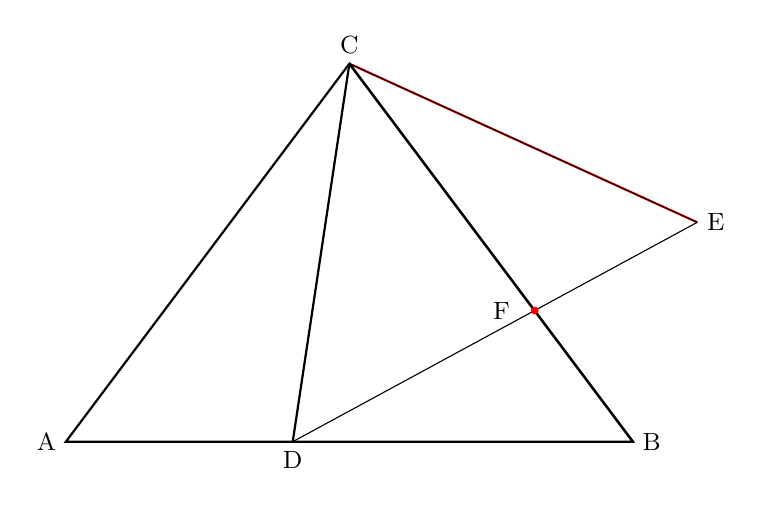
\begin{tikzpicture}[scale=1.2]
            % 三角形ABC构造
            \coordinate (A) at (0,0);
            \coordinate (B) at (6,0);
            \coordinate (C) at (3,4); % 顶点C在上方,构成等腰三角形

            \draw[thick] (A) -- (B) -- (C) -- cycle;
            \node[left] at (A) {\small A};
            \node[right] at (B) {\small B};
            \node[above] at (C) {\small C};

            % 点D在AB边上(可调位置)
            \coordinate (D) at ($(A)!0.4!(B)$);
            \node[below] at (D) {\small D};
            \draw[thick] (C) -- (D);

            % 绕点C逆时针旋转CD得到CE,使∠ACB = ∠DCE
            % 计算CD向量
            % 计算CD向量并旋转
            % \path let \p1 = (C), \p2 = (D) in
            % \pgfextra{
            %     \pgfmathsetmacro{\dx}{\x2 - \x1}
            %     \pgfmathsetmacro{\dy}{\y2 - \y1}
            %     \pgfmathsetmacro{\angleACB}{70}
            %     \pgfmathsetmacro{\cosAngle}{cos(\angleACB)}
            %     \pgfmathsetmacro{\sinAngle}{sin(\angleACB)}
            %     \xdef\ex{\cosAngle*\dx - \sinAngle*\dy}
            %     \xdef\ey{\sinAngle*\dx + \cosAngle*\dy}
            % };
            % \coordinate (E) at ($(C) + (\ex pt, \ey pt)$);
            % \draw[thick,red,rotate around={106:(C)}] (C) -- (D) node[right] {G};

            \pgfmathsetmacro{\angleACB}{74} % 旋转角度
            \path let \p1 = (C), \p2 = (D) in
            coordinate (E) at
            ($(C)+({cos(\angleACB)*(\x2-\x1) - sin(\angleACB)*(\y2-\y1)},
                {sin(\angleACB)*(\x2-\x1) + cos(\angleACB)*(\y2-\y1)})$);
            \draw[thick,red] (C) -- (E);






            \node[right] at (E) {\small E};



            \draw (C) -- (E);

            % 连接DE并与BC交于F
            \draw (D) -- (E);
            \draw[thick] (B) -- (C);
            \coordinate (F) at (intersection of D--E and B--C);
            \filldraw[red] (F) circle (1pt);
            \node[xshift = -12pt] at (F) {\small F};
        \end{tikzpicture}
    \end{minipage}

\end{center}
\textbf{解:}
设 $AD = x$,则 $DB=6-x$,\newline
$\triangle ACD \sim \triangle BDF$,\newline
$\frac{AC}{BD} = \frac{AD}{BF}$,\newline
$\frac{5}{6-x} = \frac{x}{BF}$,\newline
$BF = \frac{6x-x^2}{5}$,\newline
$BF$最大值为 $\frac{9}{5}$。\newline
$\therefore \min CF = \frac{16}{5}$。
\begin{tcolorbox}[colback=blue!5!white,colframe=blue!75!black,title=提示]
    最值问题,以前都是靠两点之间线段最短、垂线段最短,这里是靠方程来解决。这也是一个很好的方法。
\end{tcolorbox}
\subsubsection{比相关}
如图,在三角形 $\triangle ABC$ 中,$AB = AC$,$\angle B = 30^\circ$,点 $D$、$E$ 是边 $BC$ 上的两个动点,且满足 $\angle DAB = 60^\circ$。若以 $BD$、$DE$、$EC$ 的长度为边长构成一个直角三角形,则 $BD : EC$ 的可能值是:
\begin{center}


    \begin{tasks}(4) % 括号内数字表示每行最多几个选项
        \task[A.] $2 : 1$
        \task[B.] $\sqrt{3} : 1$
        \task[C.] $\sqrt{3} : 2$
        \task[D.] $2 : \sqrt{3}$
    \end{tasks}
\end{center}








\end{document}